\section{Drift Chamber Tracking System Performance}


\subsection{Chamber Lifetime}
\label{choper}

\hskip 0.15 in 
In order to satisfy the statistical requirements of the experimental program, 
a critical design goal for CLAS is the ability to make routine measurements 
with electron beams giving luminosities of up to 
1$\times$10$^{35}$~cm$^{-2}$s$^{-1}$.  The tolerable luminosity in CLAS is 
generally set by the large flux of M{\o}ller electrons and low-energy photons 
produced from the targets by the multi-GeV incident electron beam.  This 
constraint is severe for the drift chambers since they are close to the 
target. Particularly for the R1 chambers, the large flux of 
particles limits the luminosity in two ways.  First, a large number of 
background-related hits in the chambers reduces the track reconstruction 
efficiency.  The working assumption is that the analysis software can tolerate 
no more that a 5$\%$ accidental chamber occupancy in order to successfully 
reconstruct charged-particle tracks.  Second, the effects of sustained high 
luminosities are unfavorable for long chamber lifetimes.  Aging correlates 
directly with the currents generated in the chambers.

We have not yet observed any sign of aging in the drift chambers.
For the previous CLAS chambers, we used the same gas mixture and ran at a
similar gain and the chambers lasted more than 10 years with no indication
of aging.  We expect the present
chambers to perform well for at least 10 years.


\subsection{Efficiency}

\hskip 0.15in
The probability of reconstructing a track due to a charged particle within
our fiducial volume is referred to as the ``tracking efficiency''.
There are three categories of inefficiency: the ``intrinsic layer inefficiency'',
the ``background-related inefficiency'' and the ``malfunction related 
inefficiency''.

The layer efficiency is the probability that a
good hit is recorded in a wire layer through which the track has passed, based on 
the evidence from all other layers in the superlayer.  This is called the 
``excluded-layer method''.  The layer efficiency is a measure of the intrinsic drift 
cell efficiency for the particular choice of gas mixture, high-voltage set point, and 
discriminator level.  

In the section on commissioning we discussed our `high voltage plateau'.
We took data at successively higher values of high voltage and measured the
layer efficiency at each point.  We set the high-voltage operating points such that
the average layer efficiency is $>$98$\%$. 
Fig.~\ref{hit-effcy-vs-doca} reveals that a large contribution to the 2$\%$ inefficiency comes 
from tracks that pass close to the sense wire.  These tracks give rise to signals 
that have low pulse height and long duration, and thus may escape detection.

\subsection{Track Resolution}

\hskip 0.15in
The tracking resolution is the spread in the reconstructed
momenta and angles of the charged-particle tracks relative to their true values.
These tracking uncertainties arise from three primary sources: multiple scattering 
in the material along the particle trajectory, geometric misalignments of the separate 
tracking chambers or lack of knowledge 
of the true value of the traversed magnetic field strength, and finally, the  
single-wire resolution.  

Fig.~\ref{zvertex} is an illustration of the effect of finite track resolution
on the reconstruction of the beam-target vertex.
The reconstructed beam
vertex position is plotted versus the dimension along the beam
line for data with the beam incident upon an empty 
target cell.  These data were acquired for charged tracks in the angular range from 
75$^{\circ}$ to 105$^{\circ}$.  The peaks at the $z$-positions -2.0~cm and 1.8~cm 
correspond to the entrance and exit windows of the 3.8-cm long target, and the peak 
at $z=3.8$~cm corresponds to a 20-$\mu$m aluminum calibration foil.  The width of 
each peak is about $\sigma$=2~mm.  As the R1 wires illuminated in this reconstruction 
are about 0.5~m from the target, this peak width roughly translates into an angular 
uncertainty at the position of R1 of about 4 mrad.  Again, this resolution includes
contributions from the intrinsic system resolution, chamber misalignment and magnetic
field uncertainties, and multiple scattering.
  
%%%%%%%%%%%%%%%%%%%%%% Figure : Z-Vertex Resolution %%%%%%%%%%%%%%%%%%%%%%%%%%
\begin{figure}[htpb]
\vspace{5cm} 
\special{psfile=tge1c.eps hscale=52 vscale=42 hoffset=-30 voffset=-100}
\caption{\small{Reconstructed beam-target vertex position for an electron beam
incident upon an empty target cell.  The three peaks correspond to the
target entrance and exit windows and an aluminum calibration foil.}}
\label{zvertex}
\end{figure}
% resolution: pos. -1.962+/-0.218cm ; 1.765+/-0.198cm ; 3.843+/- 0.206cm
%%%%%%%%%%%%%%%%%%%%%%%%%%%%%%%%%%%%%%%%%%%%%%%%%%%%%%%%%%%%%%%%%%%%%%%%%%%%%%


As a consistency check Fig.~\ref{elastic} shows for one sector the mass 
distribution of the hadronic final state $W$ for 2.4 and 4.0~GeV e-p scattering.
The elastic-peak width ($\sigma_{2.4} \approx$12~MeV, $\sigma_{4.0} 
\approx$16~MeV) provides a measure of the mass resolution of the tracking system.
The part of the mass resolution arising from spatial resolution of the tracking
chambers is expected to grow with increasing momentum; thus the
elastic peak widths at 2.4 and 4.0~GeV are consistent.

%%%%%%%%%%%%%%%%%%%%%% Figure : Angular and Momentum Resolution %%%%%%%%%%%%%%
\begin{figure}[htpb]
\vspace{5.5cm} 
\special{psfile=elastic_1.eps hscale=45 vscale=50 hoffset=-10 voffset=-135}
\caption{\small{Reconstructed 2.4 (left) and 4~GeV (right) $W$ distribution for 
one sector showing the e-p elastic peak and inelastic excitations.}}
\label{elastic}
\end{figure}
%%%%%%%%%%%%%%%%%%%%%%%%%%%%%%%%%%%%%%%%%%%%%%%%%%%%%%%%%%%%%%%%%%%%%%%%%%%%%%


The various contributions to the overall system resolution can be studied
through detailed detector simulations as well as CLAS data.  For the overall
track fit through a given sector, an additional uncertainty of 300~$\mu$m for 
R1, 400~$\mu$m for R2, and 450~$\mu$m for R3 is added in quadrature to the
measured single-wire resolution (see next sub-section) to account for chamber 
misalignments, uncertainties in the CLAS magnetic field, and multiple scattering.
The final $\chi^2$ distribution is shown in Fig.~\ref{chi2fit} for the 
full fit through all six superlayers of each sector.


%%%%%%%%%%%%%%%%%%%%%% Figure : chi^2 distribution   %%%%%%%%%%%%%%%%%%%%%%%%%
\begin{figure}[htpb]
\vspace{5cm} 
\special{psfile=chi2e1b.eps hscale=50 vscale=40 hoffset=-25 voffset=-85}
\caption{\small{$\chi^2$ distribution per degree of freedom of the overall track 
fit using the residual sigmas for each of the drift chamber Regions and an 
additional error to account for chamber misalignments and imperfections of the
magnetic-field maps.}}
\label{chi2fit}
\end{figure}
%%%%%%%%%%%%%%%%%%%%%%%%%%%%%%%%%%%%%%%%%%%%%%%%%%%%%%%%%%%%%%%%%%%%%%%%%%%%%%

\subsection{Chamber Resolution}

\hskip 0.15in
The intrinsic chamber resolution, or single-wire resolution, is a measure
of the uncertainty between the DOCA of the track and the distance as
calculated from the time of the wire hit.  The excluded-layer fitting method 
has been used to estimate the single-wire resolution within a given superlayer.  
Tracks fitted to all hits except those on the excluded layer are projected to 
determine the intercept in the excluded layer.  The fit residual is the difference 
between the fitted DOCA of the track and the value of DOCA as calculated from the 
time of the hit in the excluded layer.  The variance of this residual distribution 
is the quadratic sum of the single-wire resolution and the track position uncertainty 
at the excluded layer.  This variance over-estimates the single-wire resolution.
Since there are six layers per superlayer and layer 3 is excluded from the fit,
this amounts to a $10 - 15\%$ over-estimate.

Fig.~\ref{resolution-vs-doca} shows the width of the track-hit residual distribution plotted versus DOCA for 
each of the different chamber Regions.  The single-wire resolution worsens near the 
wire and also at the outer edge of the cell.  This arises due to finite cluster sizes 
due to the Poisson distribution of ion-pair production along the path of the primary ion 
near the sense wire along with time walk effects and the divergent nature of the electric
field lines near the field wire.  The average single-wire resolution in the middle 
portion of the cell for each Region is presently about 200 to 250~$\mu$m.  The whole-cell 
average is about 310, 315 or 380~$\mu$m for R1, R2, and R3, respectively.

The bottom sub-figure is a histogram of the tracks' DOCA distribution.  It is approximately flat as
expected, since the particle luminosity is approximately constant over the small solid
angle of a single drift cell.  It shows a dip at zero, which is a real effect and is
due to a spreading out of the arrival time of ionized electrons when the track is
very close to the wire.
%%%%%%%%%%%%%%%%%%%%%%%%%%%%%%%%%%%%%%%%%%%%%%%%%%%%%%%%%%%%%%%%%%%%%%%%%
\begin{figure}[htbp]
\vspace{5cm}
\begin{picture}(50,50)
\put(-10,10)
{\hbox{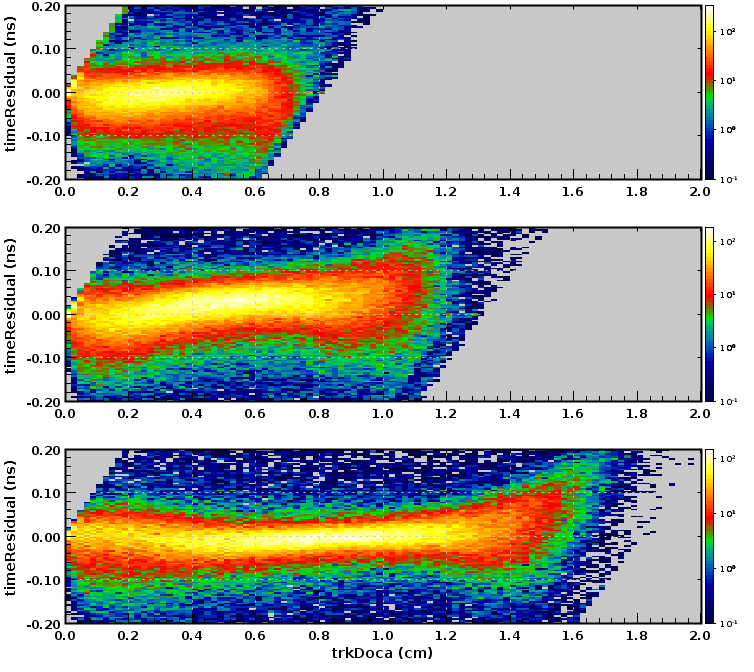
\includegraphics[width=0.35\textwidth,natwidth=610,natheight=642]{img/resolution-vs-doca.png}}}
\end{picture}
\caption{\small{Top sub-plot: Resoluton plotted versus the track DOCA (cm).  Bottom sub-plot:  The 1-d plot
of track DOCA (cm).}}
\label{resolution-vs-doca}
\end{figure}
%%%%%%%%%%%%%%%%%%%%%%%%%%%%%%%%%%%%%%%%%%%%%%%%%%%%%%%%%%%%%%%%%%%%%%%%%%%

\section{Conclusions}

\hskip 0.15in
The toroidal geometry of the CLAS spectrometer necessitated a particle-tracking 
system of unconventional design.  Design challenges and solutions include the following:

\vskip 10pt
\noindent
- The necessity to conceal inactive areas of the drift chambers within the
shadow regions of the torus cryostat resulted in very thin endplates and low-profile
wire connection schemes and on-board preamplifiers.

\noindent
- The toroidal shape of the magnet and the desire to have measurements before, within, 
and after the high-field region, resulted in the design of a `rod and ball' mounting scheme
which minimized dead areas and facilitates maintenance.

\noindent
- The fabrication of chambers that support large static wire tensions, but have thin 
endplates necessitated three endplate designs: aluminum stiffened with steel bars (R1),
G10 stiffened with steel bars (R2) and Carbon fiber plates filled with foam and reinforce
with Carbon-fiber posts and close-out plate (R3). 

\noindent
-The need for precise tracking in a system with non-saturated drift velocity 
(necessitated by the requirements of large drift distances, non-flammable gas mixtures 
and low-gain operation) resulted in a semi-automated calibration and monitoring software 
package.

\vskip 10pt
The CLAS drift chamber system has been in routine operation since Spring, 2017. 
The system has reached its design goals of 
high-luminosity operation (1$\times$10$^{35}$~cm$^{-2}$s$^{-1}$) in a 
high-flux electromagnetic reaction environment, with very good track 
reconstruction efficiency over a large range of angles and 
magnetic fields.  The single-wire efficiency is greater than $98\%$ and the
single-wire resolution is about 330~$\mu$m averaged over all drift distances and
all 18 chambers, with each chamber showing a characteristic 250~$\mu$m resolution 
in the cell center.

\vskip 10 pt

{\large{\bf Acknowledgments}}

\vskip 10pt

The authors wish to thank the crews of wire stringers and technicians who 
participated during the sector construction at the University of Pittsburgh,
Old Dominion University, and Jefferson Laboratory, as well as the support of 
the technicians involved with installation of the detectors into CLAS.  The
authors also thank S. Corneliussen for his careful reading of the draft.  This
work was supported in part by DOE contract DE-AC05-84ER40150, DOE grants 
DE-FG02-87ER40315, DE-FG05-94ER40859, DE-FG02-96ER40960, DE-FG02-96ER40980, 
and NSF grant NSF-PHY-9412479.

\vskip 10pt

\noindent
$^{\dagger}$Present address : Syncsort Inc, Woodcliff Lake, NJ 07695 USA.

\noindent
$^{\ddagger}$Present address : Los Alamos National Laboratory, Los Alamos, NM
87545 USA.


